\documentclass[12pt]{article}
\usepackage{amsmath, amssymb, amsthm}
\usepackage{graphicx}
\usepackage{hyperref}
\usepackage{float}
\usepackage{geometry}
\geometry{margin=1in}

\title{CS461 Homework 2}
\author{Mannan Shukla}
\date{Due: October 20, 2024}

\begin{document}

\maketitle

\section*{Problem 1: Linear Models and MMSE Regression}

\subsection*{1.1 Data Matrix}
Write out the data matrix \( \Phi \) based on the given data points.

\[
\Phi = \begin{bmatrix}
1 & 4 & 1 & 1 \\
1 & 7 & 0 & 2 \\
1 & 10 & 1 & 3 \\
1 & 13 & 0 & 4
\end{bmatrix}
\]

\subsection*{1.2 Exact or MMSE Solution}
We can figure out whether or not not the normal equation will yield an exact solution based on the invertibility of $\Phi^T \Phi$. If $\Phi^T \Phi$ is invertible, the equation can be solved without the need for any estimation. To find invertibility, we need to find its determinent. When calculating this with numpy, the determinent is 0. Therefore, $\Phi^T \Phi$ is not invertible and we have to use MMSE estimation because there is no way to calculate an exact solution.

\subsection*{1.3 Solving the Normal Equation}
Since $\Phi^T \Phi$ is not invertible, we cannot directly solve the normal equation. Normally, the equation is:
\[
(\Phi^T \Phi) \mathbf{w} = \Phi^T \mathbf{y}
\]
Because $\Phi^T \Phi$ is singular, we use Singular Value Decomposition (SVD) to calculate the pseudoinverse, allowing us to rearrange the equation as:
\[
\mathbf{w} = (\Phi^T \Phi)^{-1} \Phi^T \mathbf{y} = \Phi^+ \mathbf{y}
\]
After solving this using SVD, we find:
\[
\mathbf{w} = [0, 3, 3, 1]
\]

\subsection*{1.4 Comparing the Models}
The weights are different because the data matrix \(\Phi\) is rank-deficient, meaning it has linearly dependent columns. This makes \(\Phi^T \Phi\) non-invertible, which prevents the normal equation from finding a unique, exact solution. Instead, the calculation uses the pseudoinverse to obtain an approximation of the weights.
\\ \\
Since the pseudoinverse provides the best-fit solution in a least-squares sense, it does not recover the exact original weights. Essentially, there isn’t enough independent information in the data to recreate the exact original model.

\subsection*{1.5 Adding New Data Points}
After adding the four additional data points, the new data matrix was used to recompute the weights \( \mathbf{w} \). The result is: $\mathbf{w} = [-0.038, 2.995, 3.083, 1.011]$. These weights are slightly different from the previous weights \([0, 3, 3, 1]\) and very different from the actual model weights of $[1, 2, 3, 4]$.
\\ \\
This can be attributed to the fact that $\Phi$ is still rank deficient and thus there are linear depedencies. There isn't enough data and is suffering from overfitting.
\\ \\
Since there are infinitely many possible solutions, the chance of obtaining the exact original model using this method is very low, close to zero.

\subsection*{1.6 Removing Linearly Dependent Columns}
The RREF of the original data matrix \(\Phi\) is:

\[
\begin{bmatrix}
1 & 0 & 0 & \frac{1}{3} \\
0 & 1 & 0 & \frac{1}{3} \\
0 & 0 & 1 & 0 \\
0 & 0 & 0 & 0
\end{bmatrix}
\]

The fourth column is linearly dependent, as indicated by the zero row. To address this, we removed the fourth column from \(\Phi\) to make it full rank. The recalculated weights using the normal equation were:

\[
\mathbf{w}_{\text{modified}} = \begin{bmatrix} -0.3333 \\ 3.3333 \\ 3.00 \end{bmatrix}
\]

Removing the dependent column provided a unique set of weights without needing the pseudoinverse.

\section*{Problem 2: Lagrangian Function and KKT Conditions}

\subsection*{2.1 MMSE Objective Function}
To find the optimal weights \(\mathbf{w} = (w_0, w_1)\), we minimize the MMSE objective function:
\[
J(\mathbf{w}) = \frac{1}{2} \sum_{i=1}^{2} (y_i - \mathbf{w}^T \mathbf{x}_i)^2
\]
Given the data points:
\[
d_1 = (x_1, x_2) = (1, 0), \; y = 1 \quad \text{and} \quad d_2 = (x_1, x_2) = (0, 1), \; y = 1
\]
we can express the MMSE function as:
\[
J(\mathbf{w}) = \frac{1}{2} [(1 - w_0)^2 + (1 - w_1)^2]
\]
Taking the partial derivatives with respect to \( w_0 \) and \( w_1 \), we have:
\[
\frac{\partial J}{\partial w_0} = -(1 - w_0) = 0 \Rightarrow w_0 = 1
\]
\[
\frac{\partial J}{\partial w_1} = -(1 - w_1) = 0 \Rightarrow w_1 = 1
\]
Thus, the optimal weights are:
\[
\mathbf{w} = (w_0, w_1) = (1, 1)
\]

\subsection*{2.2 Lagrangian Function}
\[
\|\mathbf{w}\|^2 = w_0^2 + w_1^2 \leq C
\]
The Lagrangian function \( \mathcal{L}(\mathbf{w}, \lambda) \) is:
\[
\mathcal{L}(\mathbf{w}, \lambda) = J(\mathbf{w}) + \lambda (\|\mathbf{w}\|^2 - C)
\]
Expanding, we have:
\[
\mathcal{L}(\mathbf{w}, \lambda) = \frac{1}{2} [(1 - w_0)^2 + (1 - w_1)^2] + \lambda (w_0^2 + w_1^2 - C)
\]

\subsection*{2.3 Solving for \( \lambda \) and \( \mathbf{w}^* \)}
To determine the optimal values of \( \lambda \) and \( \mathbf{w}^* \), we start by taking the partial derivatives of the Lagrangian \( \mathcal{L}(\mathbf{w}, \lambda) \) from Section 2.2 with respect to \( w_0 \), \( w_1 \), and \( \lambda \). Setting these derivatives equal to zero gives us the following equations:
\[
\frac{\partial \mathcal{L}}{\partial w_0} = w_0 - 1 + 2\lambda w_0 = (2\lambda + 1)w_0 - 1 = 0,
\]
\[
\frac{\partial \mathcal{L}}{\partial w_1} = w_1 - 1 + 2\lambda w_1 = (2\lambda + 1)w_1 - 1 = 0,
\]
\[
\frac{\partial \mathcal{L}}{\partial \lambda} = w_0^2 + w_1^2 - C = 0.
\]

From the first two equations, we can solve for \( w_0 \) and \( w_1 \), yielding:
\[
w_0 = w_1 = \frac{1}{2\lambda + 1}.
\]
Substituting this expression into the constraint \( w_0^2 + w_1^2 = C \) and solving for \( \lambda \), we obtain:
\[
\lambda = \frac{\sqrt{\frac{2}{C}} - 1}{2}.
\]

We proceed by substituting different values of \( C \) to calculate \( \lambda \) and \( \mathbf{w} \):

- When \( C = 0.5 \):
\[
\lambda = \frac{\sqrt{\frac{2}{0.5}} - 1}{2} = \frac{\sqrt{4} - 1}{2} = \frac{2 - 1}{2} = 0.5,
\]
\[
w_0 = w_1 = \frac{1}{2(0.5) + 1} = 0.5.
\]

- When \( C = 1 \):
\[
\lambda = \frac{\sqrt{\frac{2}{1}} - 1}{2} = \frac{\sqrt{2} - 1}{2} \approx 0.207,
\]
\[
w_0 = w_1 = \frac{1}{2(0.207) + 1} \approx 0.707.
\]

- When \( C = 2 \):
\[
\lambda = \frac{\sqrt{\frac{2}{2}} - 1}{2} = \frac{\sqrt{1} - 1}{2} = 0,
\]
\[
w_0 = w_1 = \frac{1}{2(0) + 1} = 1.
\]

- When \( C = 3 \):
\[
\lambda = \frac{\sqrt{\frac{2}{3}} - 1}{2} < 0.
\]
Since \( \lambda \) must be non-negative, we set \( \lambda = 0 \). Therefore:
\[
w_0 = w_1 = \frac{1}{2(0) + 1} = 1.
\]

\section*{Problem 3: Learning Sinusoidal Functions}

\subsection*{3.1 Implementing Ordinary MMSE Regression}
The average validation error across 5 Fold Cross Validations is 0.6874

\subsection*{3.2 Ridge Regression}
The best $\lambda*$ is 0.0001

\begin{figure}[H]
    \centering
    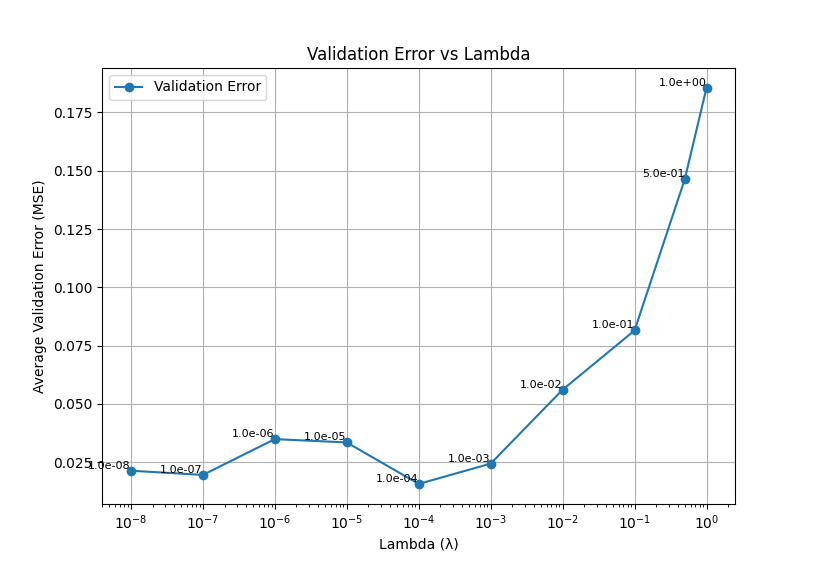
\includegraphics[width=0.7\textwidth]{ridge_regression_plot.png}
    \caption{Validation Error vs. \( \lambda \)}
\end{figure}

\subsection*{3.3 Plot the Models}

\begin{figure}[H]
    \centering
    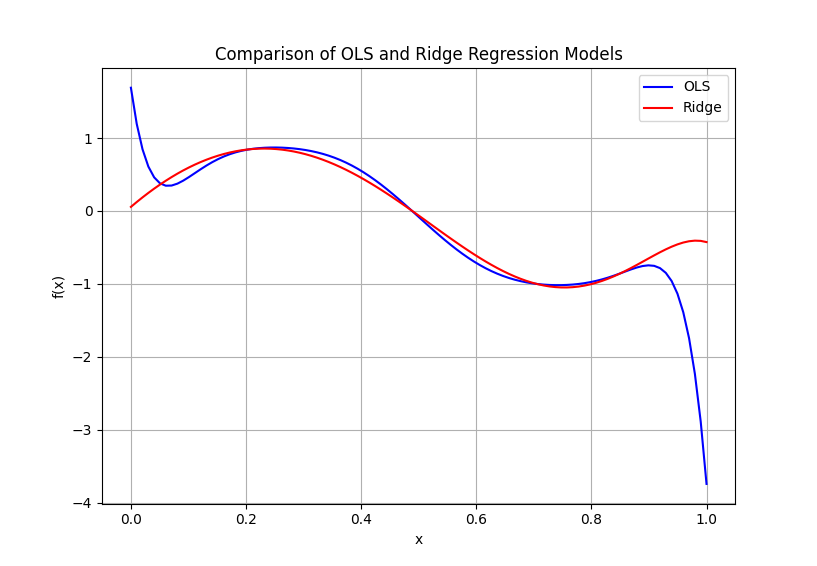
\includegraphics[width=0.7\textwidth]{3.3.png}
\end{figure}

\subsection*{3.4 Evaluate with Test Data}
OLS Test Error: 0.4447 \\
Ridge Test Error: 0.0376

\subsection*{3.5 Larger Dataset}

\begin{figure}[H]
    \centering
    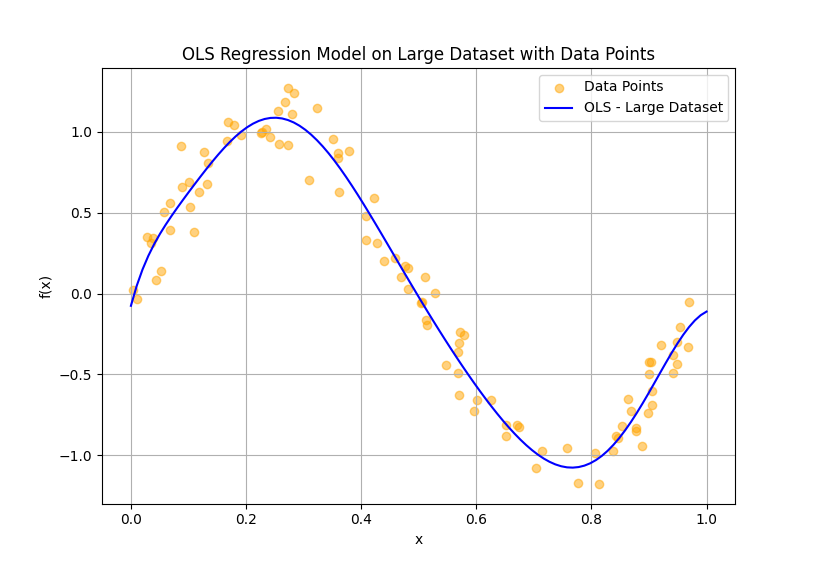
\includegraphics[width=0.7\textwidth]{3.5.png}
\end{figure}

\subsection*{3.6 Controlling Effective Complexity}
To control the effective complexity of ML problems, we can incorporate:
\begin{itemize}
\item \textbb{Regularization}, which limits the effect of high-weight coefficients, leading to smoother, less complex models
\item \textbb{Feature selection}, which limits the number of degrees the polynomial has, though we have to strike a balance to limit overfitting
\end{itemize}

\section*{Problem 4: Eigenface and Spectral Decomposition}

\subsection*{4.1 Covariance Matrix and Spectral Decomposition}
I performed the following operations using numpy:
\begin{itemize}
    \item Compute the mean vector \( \bar{x} \) to center the data.
    \item Center each image vector \( x_i \) by subtracting \( \bar{x} \) to get \( \tilde{x}_i \).
    \item Calculate the covariance matrix \( C \) using \( \tilde{x}_i \).
    \item Perform spectral decomposition \( C = E \Lambda E^T \) to extract eigenvectors (eigenfaces) and eigenvalues.
    \item Use the top \( M \) eigenvectors to approximate and reconstruct images, reducing the problem’s dimensionality.
\end{itemize}

\subsection*{4.2 Approximating the Test Image}

\begin{figure}[H]
    \centering
    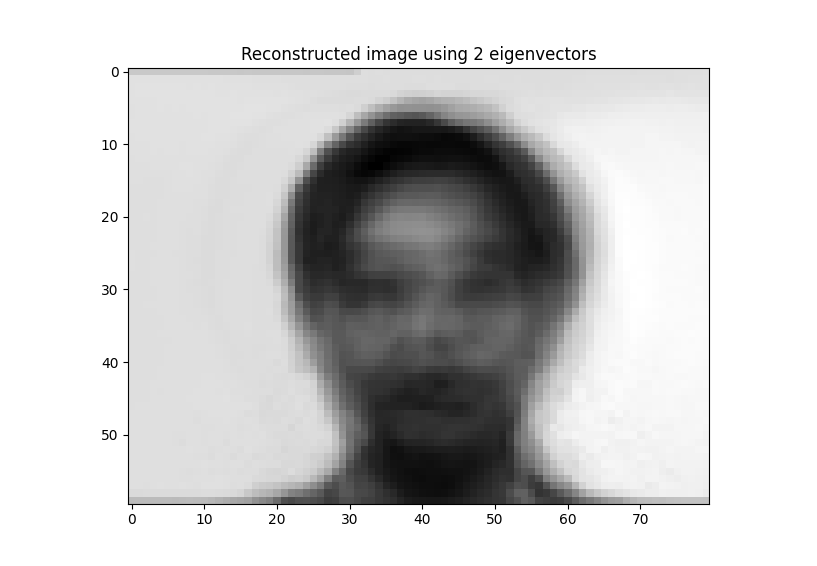
\includegraphics[width=0.3\textwidth]{eigenface_M2.png}
    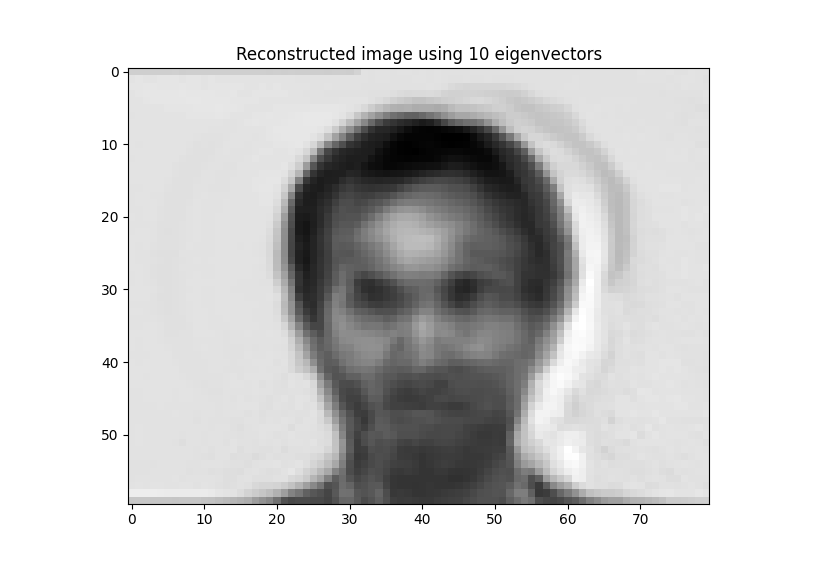
\includegraphics[width=0.3\textwidth]{eigenface_M10.png}
    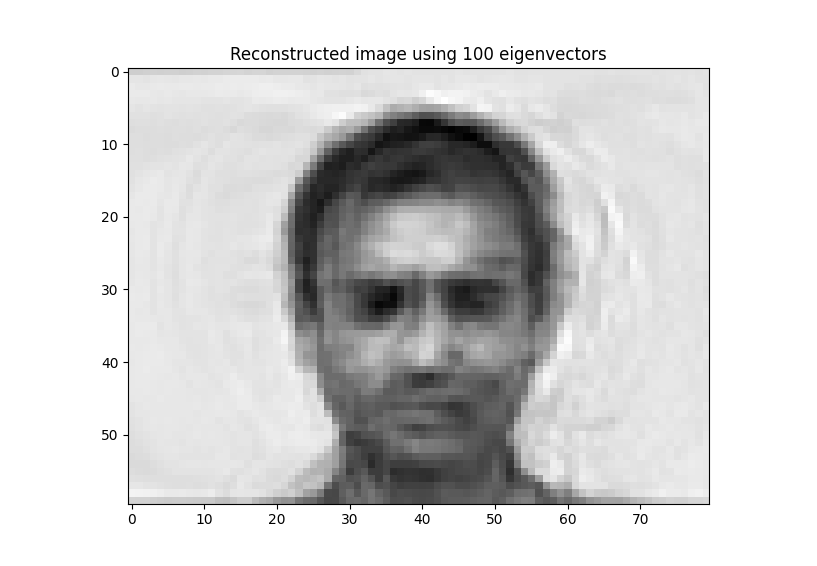
\includegraphics[width=0.3\textwidth]{eigenface_M100.png}
    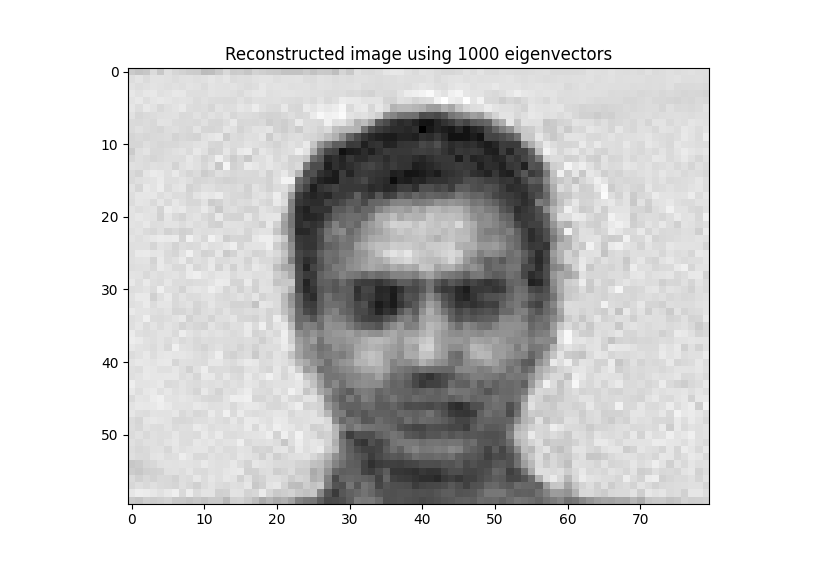
\includegraphics[width=0.3\textwidth]{eigenface_M1000.png}
    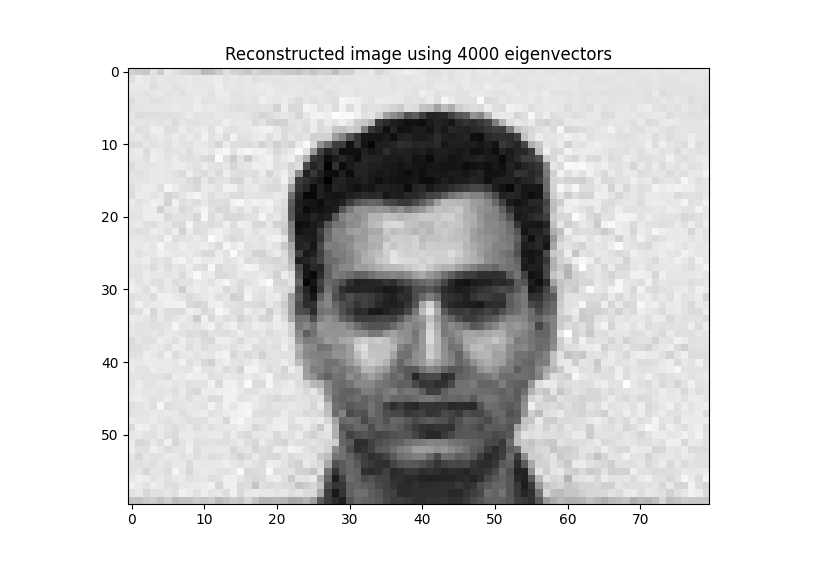
\includegraphics[width=0.3\textwidth]{eigenface_M4000.png}
    \caption{Approximations with M2, M10, M100. M1000, and M4000}
\end{figure}

\subsection*{4.3 Eigenvectors for the Largest Eigenvalues}

\begin{figure}[H]
    \centering
    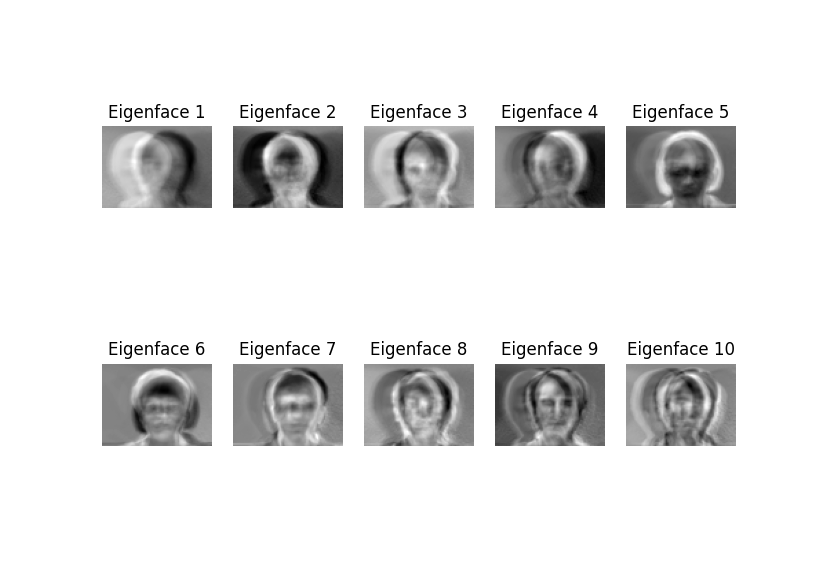
\includegraphics[width=1\textwidth]{eigenfaces_all.png}
\end{figure} 

Observations: \\
\begin{enumerate}
    \item \textbf{Eigenface 1}: Represents the broad, general features of the face, such as overall brightness and orientation. It primarily defines the basic structure of a face, including the shape of the head and its positioning.
    
    \item \textbf{Eigenface 2}: Emphasizes key facial elements like the eyes and nose, while also reflecting some differences in lighting and head tilt.
    
    \item \textbf{Eigenface 3}: Brings out finer facial distinctions, particularly the contrast between regions such as the eyes, nose, and mouth.
    
    \item \textbf{Eigenface 4}: Highlights more subtle details, focusing on features around the eyes and eyebrows, and capturing variations in the upper section of the face.
    
    \item \textbf{Eigenface 5}: Reflects differences in the mid and lower parts of the face, such as around the mouth and chin.
    
    \item \textbf{Eigenface 6}: Accentuates variations in the forehead and hairline, along with certain features near the eyes.
    
    \item \textbf{Eigenface 7}: Captures delicate structural variations, mainly around the nose and eyes, revealing subtle differences in facial form.
    
    \item \textbf{Eigenface 8}: Highlights changes in the overall contour of the face, particularly along the cheeks and jawline.
    
    \item \textbf{Eigenface 9}: Focuses on asymmetrical features, identifying discrepancies between the left and right sides of the face.
    
    \item \textbf{Eigenface 10}: Brings out very specific details, capturing minor changes around the eyes, nose, and mouth, as well as slight lighting effects or distortions.
\end{enumerate}

\section*{Problem 5: Extra Points - Year of Made Prediction}

\subsection*{5.1 Dimensional Reduction and Whitening}

\begin{figure}[H]
    \centering
    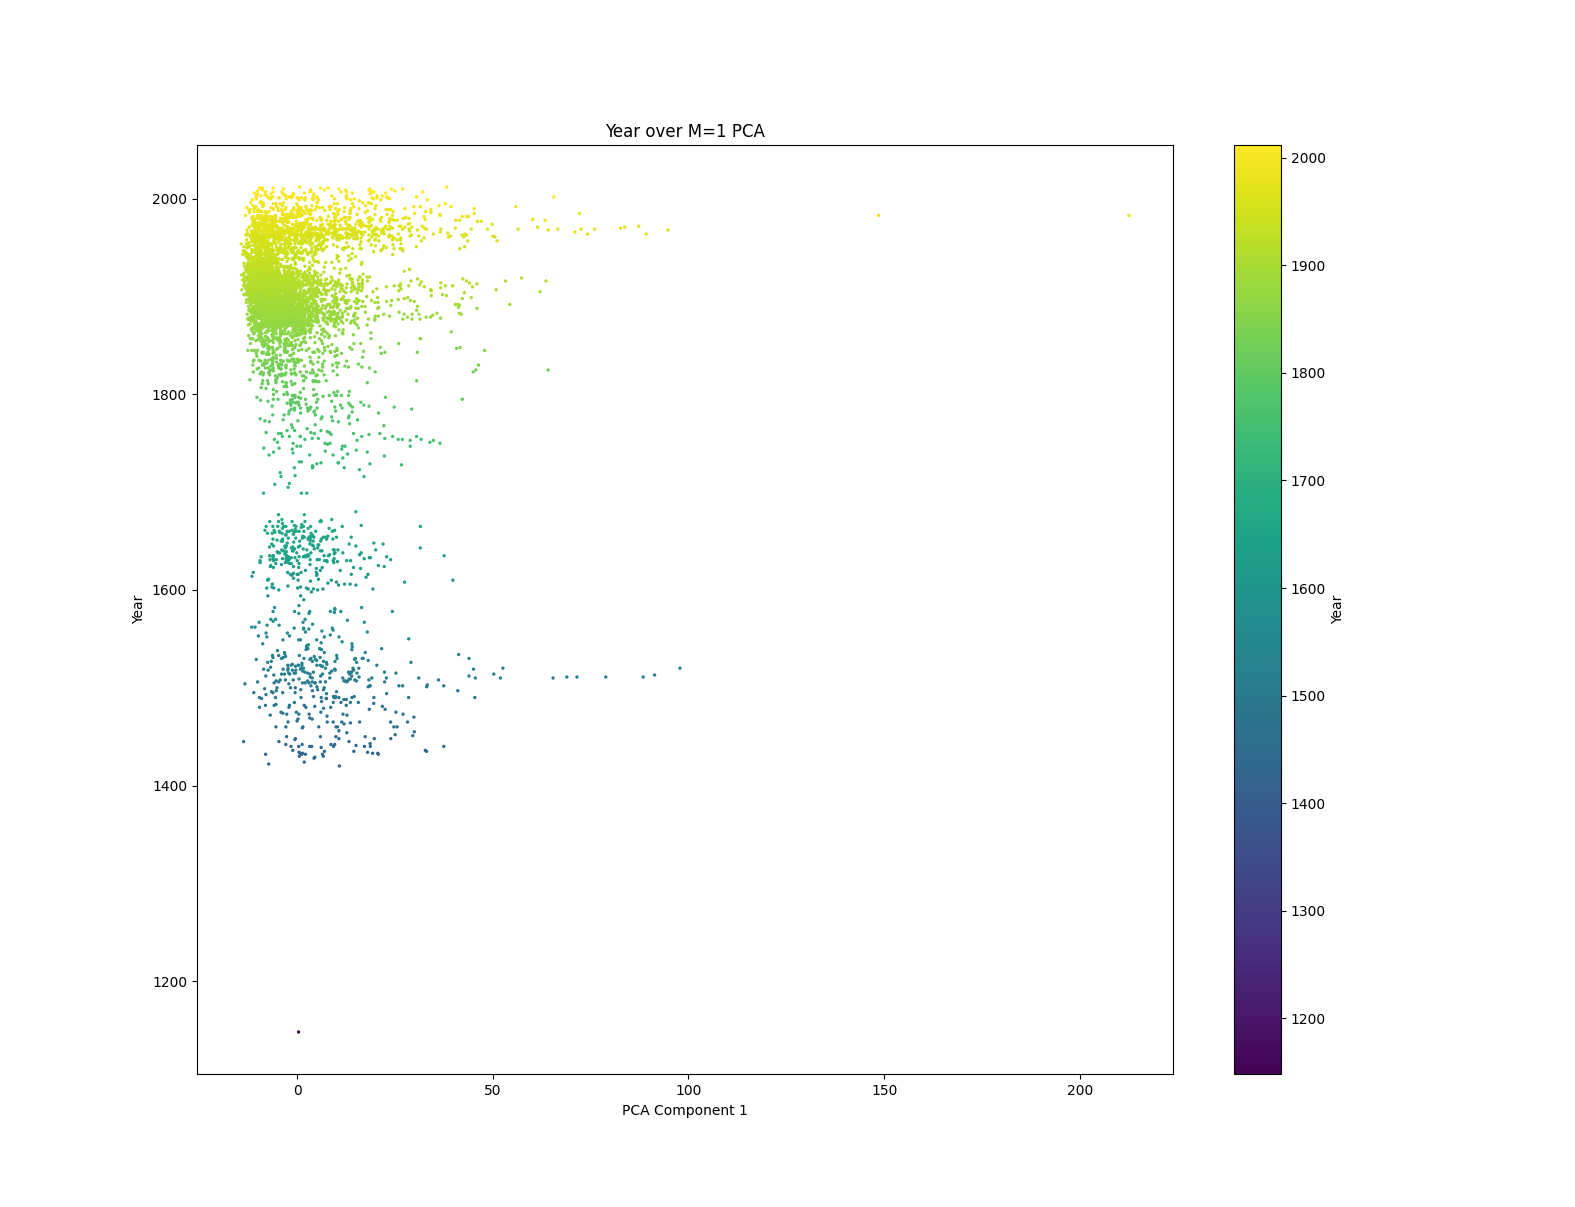
\includegraphics[width=0.5\textwidth]{plot.png}
    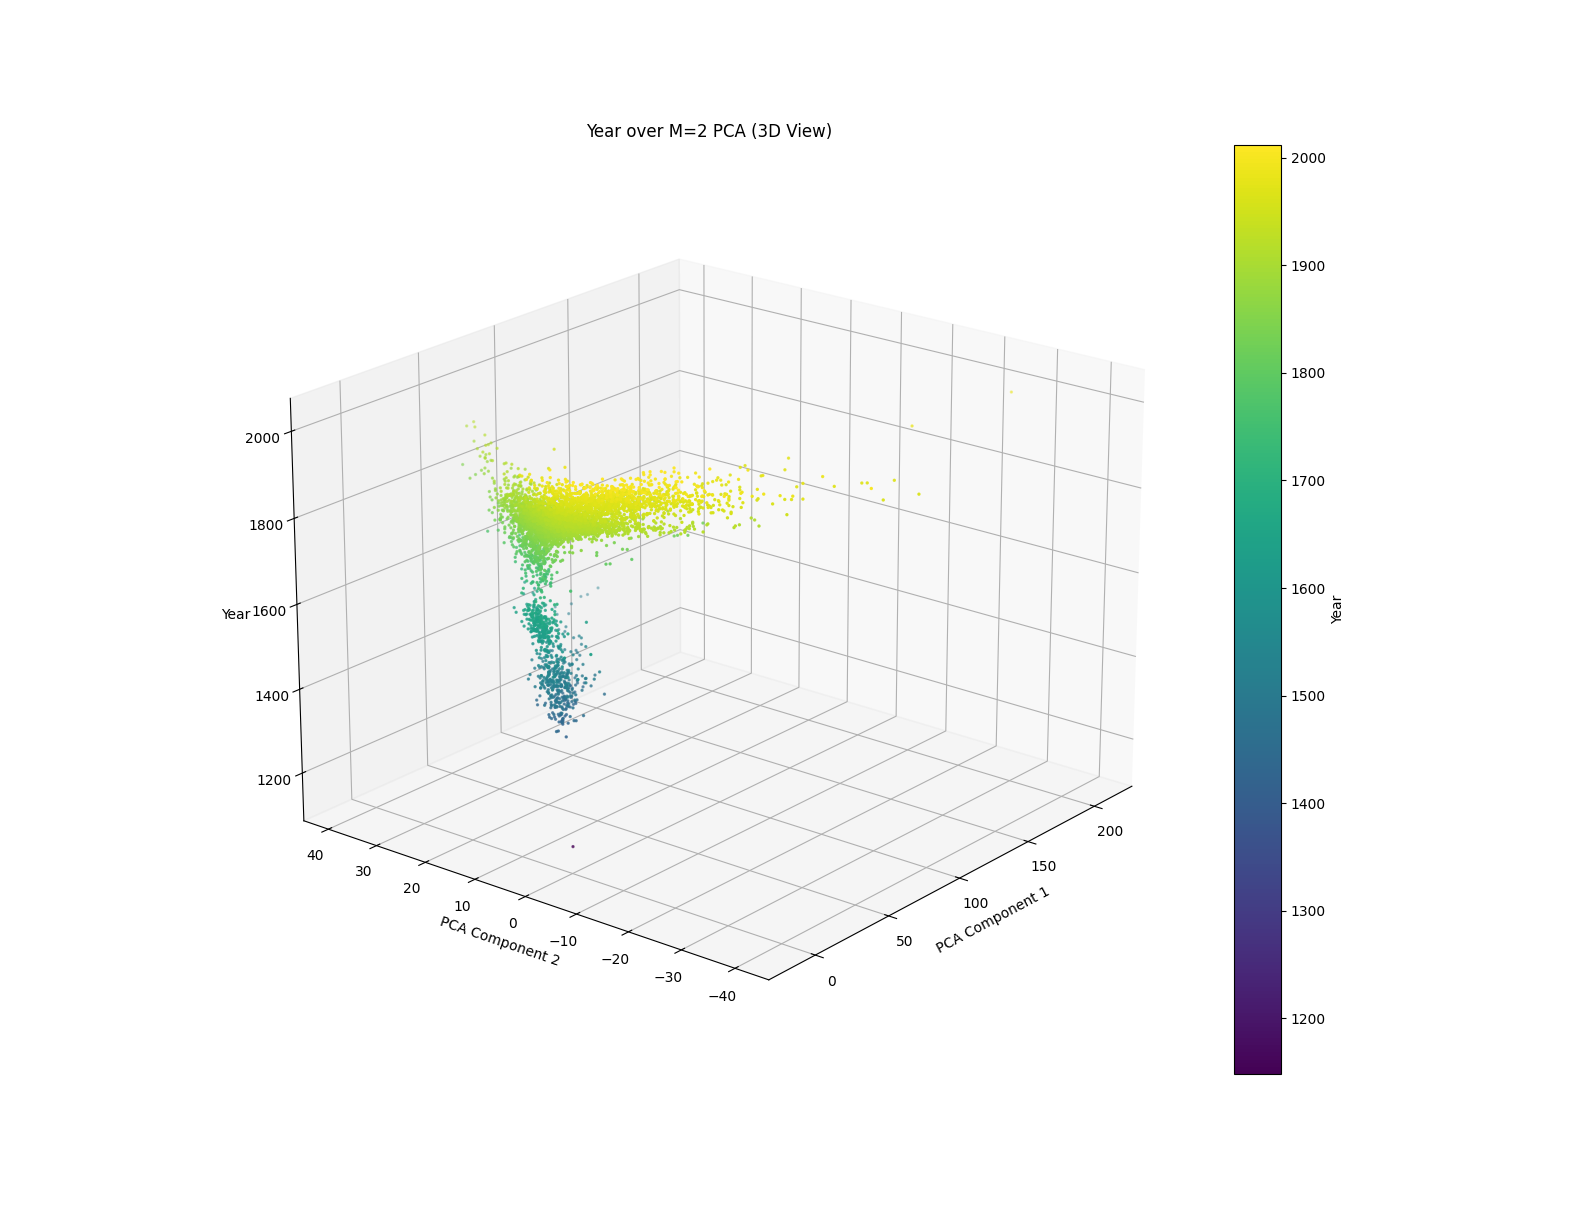
\includegraphics[width=0.5\textwidth]{plot2.png}
\end{figure} 

The 1-D PCA plot shows that a single feature cannot accurately predict the year because one x-value can correspond to multiple different years, leading to overlap and ambiguity. In contrast, the 2-D PCA plot, using two principal components, captures more variance and provides clearer separation, reducing this issue. Thus, a 2-D representation is more effective for modeling the relationship between features and the year.
\end{document}
